%!TEX root = /Users/louis/Documents/PhD/Deliverables/Thesis/thesis.tex

\section{MDE Guidelines and Methods}
\label{sec:mde_methods}
For performing model-driven engineering, new practices and processes have been proposed. Proponents of MDE have produced guidance and methods for model-driven engineering. This section discusses the guidance for MDE set out in the Model-Driven Architecture \cite{mda} and the methods described by \cite{stahl06mdsd,kelly08dsm,greenfield04software}. 

\subsection{Model-Driven Architecture (MDA)}
Model-Driven Architecture (MDA) is a software engineering framework defined by the OMG. MDA provides a set of guidelines for model-driven engineering. MDA prescribes the use of a Platform Independent Model (PIM) and one or more Platform Specific Models (PSMs).

A PIM provides an abstract, implementation-agnostic view of the solution. Successive PSMs provide increasingly more implementation detail. Inter-model mappings are used to forward- and reverse-engineer these models, as depicted in
Figure \ref{fig:mda}.

\begin{figure}[htbp]
  \begin{center}
    \leavevmode
    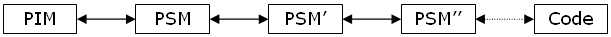
\includegraphics[scale=0.5]{2.Background/images/PIMs_and_PSMs.png}
  \end{center}
  \caption{Interactions between a PIM and several PSMs.}
  \label{fig:mda}
\end{figure}

The crucial difference between MDA and related approaches, such as round-trip engineering (in which models and code are co-evolved to develop a system), is that traditional round-trip engineering uses some manual transformations, whereas MDA prescribes automated transformations between PIM and PSMs.

McNeile \cite{mcneile03mda} identifies two ways in which engineers are utilising MDA. Both interpretations begin with a PIM and vary in the way they are used to produce executable code:

\begin{itemize}
 \item \textbf{Translationist}: The PIM is used to generate code directly using a sophisticated code generator. Any intermediate PSMs are internal to the code generator. No generated artefacts are edited manually.
 \item \textbf{Elaborationist}: Any generated artefacts (such as PSMs, code and documentation) can be augmented with further details of the application. To ensure that all models and code are synchronised, tools must allow bi-directional transformations.
\end{itemize}

Translationists must encode behaviour in their PIMs \cite{mellor02executable}, whereas elaborationists have a choice, frequently electing to specify behaviour in PSMs or in code \cite{kleppe03mda}.

The MDA prescribes a set of standards for MDE. The MDA allocates standards to one of four tiers, representing different levels of model abstraction. Members of each tier are instances of the members of parent tiers. These tiers can be seen in Figure \ref{fig:mda-pyramid}, and a short discussion based on \cite[Section 8.2]{kleppe03mda} follows.

\begin{figure}[htbp]
  \begin{center}
    \leavevmode
    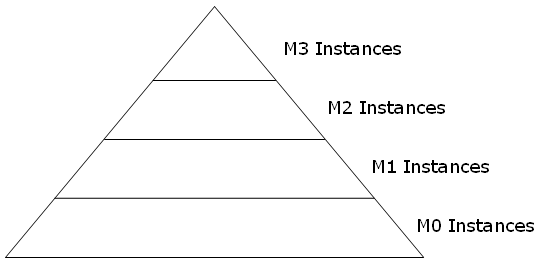
\includegraphics[scale=0.5]{2.Background/images/mda-pyramid.png}
  \end{center}
  \caption{The tiers of standards used as part of MDA.}
  \label{fig:mda-pyramid}
\end{figure}

The base of the pyramid, tier M0, describes the domain (real-world). When modelling a business, this tier is used to describe items of the business itself, such as a real customer or an invoice. When modelling software, M0 instances describe the software representation of such items. M1 contains a model of the concepts in M0, for example a customer may be represented as a class with attributes. The M2 tier describes the model of the modelling language used to describe elements of M1. For example, if UML \cite{uml212} were used to describe concepts as classes in the M1 tier, M2 would contain the UML metamodel. Finally, M3 is the meta-metamodel layer, which provides a description of the metamodel used in M2. M3 is necessary to permit reasoning about metamodels (such as the UML), and to enable tool standardisation. The OMG defines the Meta-Object Facility (MOF) \cite{mof} as the sole inhabitant of the M3 tier.


\subsection{Methods for MDE}
Several methods to MDE are prevalent today. In this section, three of the most established are discussed: Architecture-Centric Model-Driven Software Development \cite{stahl06mdsd}, Domain-Specific Modelling \cite{kelly08dsm} and Microsoft's Software Factories \cite{greenfield04software}. All three methods have been defined from a pragmatic standpoint, and have been used repeatedly to solve problems in industry. The methods vary in the extent to which they follow the guidelines set out by MDA.

\subsubsection{Architecture-Centric Model-Driven Software Development}
Model-Driven Software Development is the term given to MDE by in \cite{stahl06mdsd}. The style of MDE that Stahl et al. describe, \textit{architecture-centric model-driven software development} (AC-MDSD), focuses on generating the infrastructure of large-scale applications. For example, a typical J2EE application contains concepts (such as EJBs, descriptors, home and remote interfaces) that ``admittedly contain domain-related information such as method signatures, but which also exhibit a high degree of redundancy'' \cite{stahl06mdsd}. It is this redundancy that AC-MDSD seeks to remove by using code generators, requiring only the domain-related information to be specified.

AC-MDSD applies more of the MDA guidelines than the other methods discussed below. For instance, AC-MDSD supports the use of a general-purpose modelling language for specifying models. \cite{stahl06mdsd} utilise UML in many of their examples, which demonstrate how AC-MDSD may be used to enhance the productivity, efficiency and understandability of software development. In these examples, models are annotated using UML profiles to describe domain-specific concepts.


\subsubsection{Domain-Specific Modelling}
\cite{kelly08dsm} present a method for MDE termed Domain-Specific Modelling (DSM). DSM is based on the translationist interpretation of MDA; DSM seeks to translate models containing concepts from the problem domain to full code. In motivating the need for DSM, Kelly and Tolvanen state that large productivity gains were made when third-generation programming languages were used in place of assembler, and that no paradigm shift has since been able to replicate this degree of improvement. Tolvanen\footnote{Tutorial on Domain Specific Modelling for Full Code Generation at the Fourth European Conference on Model Driven Architecture (ECMDA), June 2008, Berlin, Germany.} notes that DSM focuses on increasing the productivity of software engineering by allowing developers to specify solutions by using models that describe the application domain.

To perform DSM, expert developers define:

\begin{itemize}
 \item \textbf{A domain-specific modelling language}: allowing domain experts to encode solutions to their problems.
 \item \textbf{A code generator}: that translates the domain-specific models to executable code in an existing programming language.
 \item \textbf{Framework code}: that encapsulates the common areas of all applications in this domain.
\end{itemize}

As the development of these three artefacts requires significant effort from expert developers, Tolvanen\footnotemark[\value{footnote}] states that DSM should only be applied if more than three problems specific to the same domain are to be solved.

Tools for defining domain-specific modelling languages, editors and code generators enable DSM \cite{kelly08dsm}. Reducing the effort required to specify these artefacts is key to the success of DSM. In this respect, DSM resembles a programming paradigm popular in the \textit{domain-specific language} (DSL) community, termed \textit{language-oriented programming} (LOP), which also requires tools to simplify the specification of new languages. DSLs and LOP are discussed further in Section \ref{sec:mde_related}.

Throughout \cite{kelly08dsm}, examples from industrial partners are used to illustrate that DSM can greatly improve developer productivity. Unlike MDA, DSM seems to be optimised for increasing productivity, and less concerned with portability or maintainability. Therefore, DSM is less suitable for engineering applications that frequently interoperate with -- and are underpinned by -- changing technologies.

\subsubsection{Microsoft Software Factories}
Greenfield \cite[pg159]{greenfield04software} states that industrialisation of the automobile industry has addressed problems with economies of scale (mass production) and scope (product variation). Software Factories, a software engineering method developed at Microsoft, seek to address problems with economies of scope in software engineering by borrowing concepts from product-line engineering. Greenfield \cite{greenfield04software} argues that, unlike many other engineering disciplines, software development requires considerably more development effort than production effort in that scaling software development to account for scope is significantly more complicated then mass production of the same software system.

The Software Factories method \cite{greenfield04software} prescribes a bottom-up approach to abstraction and re-use. Development begins by producing prototypical applications. The common elements of these applications are identified and abstracted into a product-line. When instantiating a product, models are used to specify product variance (e.g. by selecting particular product features). To generate these models, tools for use with Software Factories provide mechanisms for defining wizards and feature-based configuration selection dialogues. By contrast, DSM relies upon the use of concrete syntax for producing models that describe product variance. By providing explanations that assist in making decisions, the wizards used in Software Factories guide users towards best practices. Greenfield et al. state that ``moving from totally-open ended hand-coding to more constrained forms of specification [such as wizard-based feature selection] are the key to accelerating software development'' \cite[pg179]{greenfield04software}.

The Software Factories method better addresses problems of portability compared to DSM: the former provides \textit{viewpoints} into the product-line (essentially different views of development artefacts), which allow decoupling of concerns (e.g. between logical, conceptual and physical layers). Viewpoints provide a mechanism for abstracting over different layers of platform independence, adhering more closely than DSM to the guidelines provided in MDA. Unlike the guidelines provided in MDA, the Software Factories method does not insist that development artefacts be derived automatically where possible.

Finally, Software Factories prescribes the use of domain-specific languages (discussed in Section~\ref{subsec:dsls}) for describing models in conjunction with Software Factories, rather than a general-purpose modelling language, as the authors of Software Factories believe that the latter often have imprecise semantics \cite{greenfield04software}.

\subsection{Summary}
This section has discussed the ways in which process and practices for MDE have been captured. Guidance for MDE has been set out in the MDA standard, which seeks to use MDE to produce adaptable software in a productive and maintainable manner. Three methods for performing model-driven engineering have been discussed.
 
The methods discussed share some characteristics. They all require a set of exemplar applications, which are examined by MDE experts. Analysis of the exemplar applications identifies the way in which software development may be decomposed. A modelling language for the problem domain is constructed, and instances are used to generate future applications. Code common to all applications in the problem domain is encapsulated into a framework.

Each method has a different focus. AC-MDSD seeks to reduce the amount of boilerplate code being generated, particularly in enterprise applications. Software Factories concentrate on providing different viewpoints into the system, allowing different domain experts to collaborate when specifying a system. DSM aims to decrease the time taken to develop software solutions to instances of the problem domain.

Perhaps unsurprisingly, the proponents of each method for MDE recommend one or more tools, each optimised for that method (such as MetaCase for DSM). Alternative tools are available from open-source modelling communities, including the Eclipse Modelling Project, which provides -- among other tools for MDE -- arguably the most widely used MDE modelling framework today. Some of the tools used for MDE are reviewed in the sequel.